\documentclass[tikz, margin=5mm]{standalone}
\usepackage[sfdefault,light]{roboto}
\usetikzlibrary{shapes, arrows, positioning, fit, backgrounds}
\definecolor{MyGreen}{HTML}{41B3A3}
\definecolor{MyOrange}{HTML}{E27D60}
\tikzset{every picture/.style={/utils/exec={\sffamily}}}
\begin{document}
    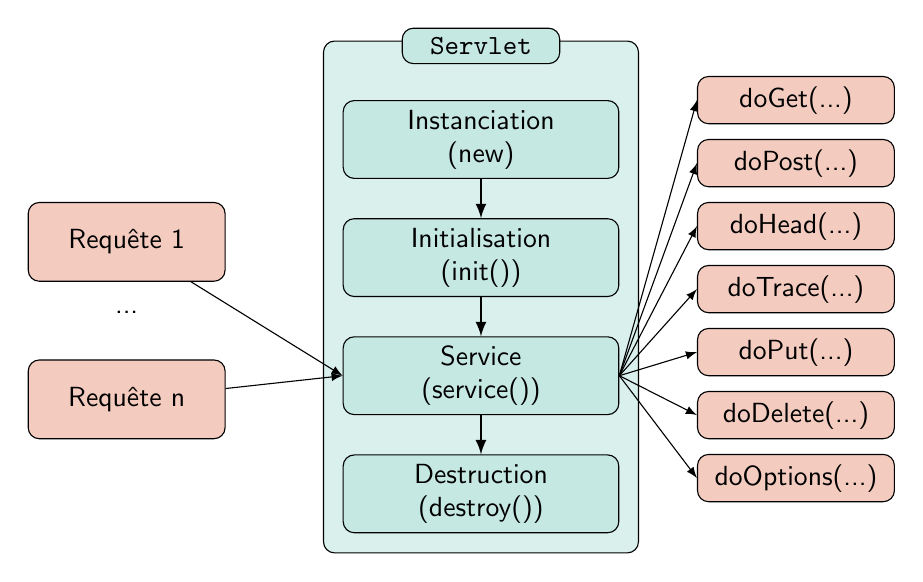
\begin{tikzpicture} [
			every node/.style={align=center,draw,rectangle,rounded corners},
			bgnode/.style={fill=MyGreen!20,minimum width=40mm,minimum height=65mm},
			serv/.style={fill=MyGreen!30,minimum width=35mm,minimum height=5mm},
			subserv/.style={fill=MyOrange!40, minimum width=25mm, minimum height=6mm},
			elt/.style={fill=MyOrange!40,minimum width=25mm,minimum height=10mm}
		]
			\node at (-1.5,0.7) [elt] (client1) {Requête 1};
			\node at (-1.5,-0.2) [draw=none] (void) {...};
			\node at (-1.5,-1.3) [elt] (client2) {Requête n};
			\node at (7,2.5) [subserv] (method1) {doGet(...)};
			\node at (7,1.7) [subserv] (method2) {doPost(...)};
			\node at (7,0.9) [subserv] (method3) {doHead(...)};
			\node at (7,0.1) [subserv] (method4) {doTrace(...)};
			\node at (7,-0.7) [subserv] (method5) {doPut(...)};
			\node at (7,-1.5) [subserv] (method6) {doDelete(...)};
			\node at (7,-2.3) [subserv] (method7) {doOptions(...)};
			\node at (3,0) [bgnode] (frame) {};
			\node at (3,2) [serv] (servinst) {Instanciation \\ (new)};
			\node at (3,0.5) [serv] (servinit) {Initialisation \\ (init())};
			\node at (3,-2.5) [serv] (servdestroy) {Destruction \\ (destroy())};
			\node at (3,-1) [serv] (servmid) {Service \\ (service())};
			\node[above=-3mm of frame, draw=black, fill=MyGreen!30, minimum width=20mm] (servname) { \texttt{Servlet}};
			\path[draw,thick,-latex] (servinst) -- (servinit);
			\path[draw,thick,-latex] (servinit) -- (servmid);
			\path[draw,thick,-latex] (servmid) -- (servdestroy);
			\path[draw,-latex] (client1) -- (servmid.west);
			\path[draw,-latex] (client2) -- (servmid.west);
			\path[draw,-latex] (servmid.east) -- (method1.west);
			\path[draw,-latex] (servmid.east) -- (method2.west);
			\path[draw,-latex] (servmid.east) -- (method3.west);
			\path[draw,-latex] (servmid.east) -- (method4.west);
			\path[draw,-latex] (servmid.east) -- (method5.west);
			\path[draw,-latex] (servmid.east) -- (method6.west);
			\path[draw,-latex] (servmid.east) -- (method7.west);
		\end{tikzpicture}
\end{document}